\section{Segnali}
Un segnale rappresenta il comportamento di grandezze fisiche in funzione di una o più variabili indipendenti. Sono monodimensionali se rappresentati da una sola variabile, per esempio il suono (continuo). I dati EEG sono multidimensionali in variazione al tempo, agli elettrodi e ai soggetti.

Le immagini in bianco e nero sono segnali bidimensionali (coordinate spaziali) e monocanale (il grigio), mentre quelle a colori hanno 3 segnali dimensionali RGB. Il campionamento corrisponde al numero di pixel, e la quantizzazione è la profondità del colore (quanti bit per la codifica). Aumentando il numero di livelli, aumenta la capacità di rappresentare l'informazione.

Se la variabile indipendente continua viene discretizzata è stato effettuato un campionamento, in cui è necessario conoscere la distanza tra i campioni (digitali). 

Il valore assunto dal segnale si definisce \textbf{ampiezza} (dipendente, codominio) mentre l'asse delle ascisse è il \textbf{dominio} (tempo o spazio). Si possono introdurre grandezze statistiche come media e varianza, indicate in modo diverso a seconda del tipo di segnale.

\begin{itemize}
	\item Continuo:
	\begin{itemize}
		\item $\mu = \lim\limits_{T \rightarrow \infty} \frac{1}{T} \int_{-\frac{T}{2}}^{\frac{T}{2}} x(t) dt$;
		\item $\mu = \frac{1}{T_1 - T_0} \int_{T_0}^{T_1} x(t) dt$;
	\end{itemize}
	\item Discreto:
	\begin{itemize}
		\item $\mu = \frac{1}{N} \sum_{i = 0}^{N - 1} x_i$.
	\end{itemize}
\end{itemize}

Il segnale digitale ha solamente una casistica di $\mu$ perché non tende mai a infinito, e il livello dell'ampiezza è diverso. Se un segnale varia, ha una componente continua DC (direct current, contributo a frequenza 0 e valore medio), e componenti AC a corrente alternata che variano in base a come il segnale fluttua intorno al valore medio.

Una forma d'onda ripetuta ha escursioni costanti, descritte da una grandezza chiamata ampiezza picco-picco $A_{pp}$. Il periodo è arbitrario.

Deviazione standard e varianza forniscono informazioni aggiuntive su quanto lontano (e con quale potenza) il segnale fluttua dal valore medio. Alla varianza è fortemente legata la potenza del rumore: un'alta varianza implica un forte rumore. \\
$\sigma^2 = \frac{1}{N - 1} \sum_{i = 0}^{N - 1} (x_i - \mu)^2$

\begin{figure}[h]
	\centering
	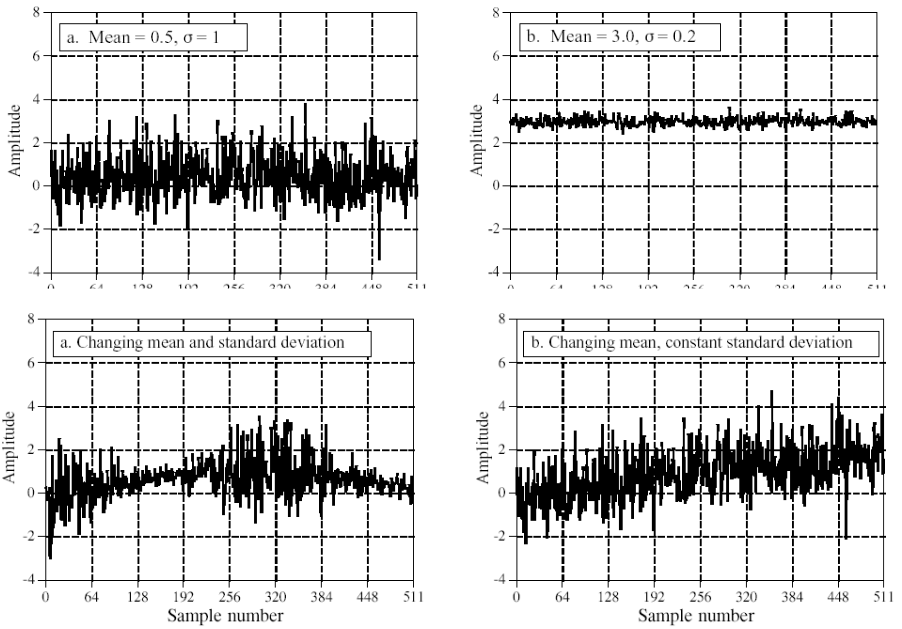
\includegraphics[scale=0.48]{Lezioni/Immagini/mediavarianza}
\end{figure}

Se media e varianza di un segnale non cambiano nel tempo, esso è stazionario. Al contrario, se il segnale varia la media sarà diversa a seconda della finestra, e la media globale non dà informazioni.

La \textbf{periodicità} indica la ripetizione del segnale nel tempo, definito appunto in periodi. Non esistono segnali puramente periodici, ma si usano approssimazioni delle forme d'onda che assume il segnale. L'inversa del periodo è chiamata \textbf{frequenza fondamentale}: $f_0 = 1/T$. 

\subsection{Segnale sinusoidale}
Un segnale sinusoidale è un seno o un coseno, monodimensionale in funzione del tempo o dello spazio.

$$A(T) = A_{med} + B \cdot \sin(2\pi ft + \varphi_0)$$
$$A_{med} = \frac{1}{T} \int_{0}^{T} A(t) dt \qquad A_{pp} = A_{max} - A_{min} \qquad B = A_{pp} / 2$$

Parametri importanti in questi casi sono \textbf{frequenza} e \textbf{fase}. 

La frequenza si misura in Hertz, e rappresenta la rapidità con cui varia l'ampiezza in un intervallo temporale $T$. La pulsazione (intera variazione di ampiezza) è proporzionale alla frequenza, si ha che $\omega = 2\pi f$. 

La fase segna l'alternarsi di positività o negatività del segnale, in particolare è significativa la fase iniziale $\varphi_0$.

$$P(t) = \abs{x(t)}^2 \qquad \text{potenza istantanea}$$
$$E_x = \int_{-\infty}^{+\infty} P(x) dt \qquad \text{energia: area di potenza istantanea}$$

Tanto più l'ampiezza si scosta dallo 0, più la potenza aumenta:
\begin{itemize}
	\item Se $E_x < \infty$ il segnale ha energia finita;
	\item Quando $E_x = \infty$ si definisce la potenza media: $P_x = \lim\limits_{T \rightarrow \infty} \frac{1}{T} \int_{-\frac{T}{2}}^{\frac{T}{2}} \abs{x(t)}^2 dt$.
\end{itemize}
Potenza media di un segnale periodico $T$: $P_x = \frac{1}{T} \int_{T} \abs{x(t)}^2 dt$

Entrambi i valori hanno una componente continua (valore medio) calcolato come il limite dell'integrale o l'integrale (segnale periodico) di $x(t)$.

\subsection{Decibel}
Il \textbf{decibel} (dB) è un'unità di misura logaritmica (quindi non lineare), in cui lo scopo del logaritmo è visualizzare meglio grandi scale di valori e avvicinarsi alla percezione umana. La misura è quindi relativa e adimensionale.

$$deciBel = dB \longrightarrow 10\log_{10} \frac{P_1}{P_2} = 20\log_{10} \frac{A_1}{A_2}$$
$$ Bel \longrightarrow \log_{10} \frac{P_1}{P_2} \qquad P = \text{potenza} \qquad A = \text{ampiezza} \qquad P \propto A^2$$

Le componenti della formula sono due pressioni, di cui il numeratore è la potenza del suono e il denominatore è la soglia minima di udibilità. La potenza è proporzionale al quadrato dell'ampiezza, quindi trasformando in scala logaritmica essa diventa un fattore moltiplicativo. $6dB$ rappresentano un raddoppio dell'ampiezza.

\subsection{Trasformazioni di segnali}
Operazioni molto comuni sono la traslazione, il cambio di scala e l'inversione temporale. \\
Se il segnale è reale, è possibile ritardarlo ma non anticiparlo.
\begin{itemize}
	\item Ritardo: fissato un tempo $t_0$, la traslazione trasforma il segnale $x(t)$ nel segnale $x(t - t_0)$;
	\item Anticipo: fissato un tempo $t_0$, la traslazione trasforma il segnale $x(t)$ nel segnale $x(t + t_0)$;
	\item Cambio di scala: dato un numero reale $a > 0$, trasformazione del segnale $f(t)$ in $f(at)$:
	\begin{itemize}
		\item Se $a > 1$ si ottiene una compressione lineare;
		\item Se $a < 1$ si ottiene un allungamento lineare;
	\end{itemize}
	\item Inversione: trasforma il segnale $f(t)$ nel segnale $f(-t)$.
\end{itemize}

Un segnale si dice pari se $f(t) = f(-t)$, dispari se $f(t) = -f(-t)$: il coseno è una funzione pari, il seno è dispari.

\subsection{Segnali continui}
Gradino: usato per selezionare la parte positiva dei segnali che tendono a $\pm \infty$. \\
Si definisce un \textbf{gradino unitario} $u(t)$:
$$u(t) = \begin{cases}
1 & \text{se } t \geq 0 \\
0 & \text{se } t < 0
\end{cases}$$

\textbf{Gradino traslato} in $t_0$: definito quando la finestra di osservazione è finita, centrata rispetto a 0. Se il segnale è fuori dall'intervallo assume valore 0:
$$u(t - t_0) = \begin{cases}
1 & \text{se } t \geq t_0 \\
0 & \text{se } t < t_0
\end{cases}$$

\textbf{Impulso rettangolare unitario} $rect(t)$:
$$rect(t) = \begin{cases}
1 & \text{se } \abs{t} \leq \nicefrac{1}{2} \\
0 & \text{se } \abs{t} > \nicefrac{1}{2}
\end{cases}$$

Quest'ultima è una funzione che forma un rettangolo di area unitaria. Generalizzando, si ha un rettangolo di altezza $A$, base $T$ e traslato in $t_0$ sostituendo nella formula unitaria $t$ con $\frac{t - t_0}{T}$ e confrontandolo con $\nicefrac{1}{2}$.
$$\abs{t - t_0} \leq T / 2 \: \begin{cases}
\text{per } (t - t_0) > 0 \qquad (t - t_0) \leq T / 2 \qquad t \leq t_0 + T / 2 \\
\text{per } (t - t_0) < 0 \qquad (t - t_0) \geq -T / 2 \qquad t \geq t_0 - T / 2
\end{cases}$$

La moltiplicazione di un segnale per un rettangolo lo approssima con segmenti verticali o orizzontali a seconda dell'asse considerato. Media e varianza non sono le stesse rispetto alla funzione originale.

Funzione \textbf{delta di Dirac} $\delta(t)$: distribuzione con rettangolo di base infinitesima e altezza infinita che abbia l'area unitaria, con la larghezza che tende a 0 e di conseguenza l'altezza che tende a infinito. 
$$\int_{-\infty}^{\infty} \delta(t) dt = 1$$
Limite dell'impulso rettangolare di base $\Delta$ per $\Delta \rightarrow 0$, dove $\Delta$ è uno scalare sull'asse $x$: 
$$\delta(t) = \lim\limits_{\Delta \rightarrow 0} \frac{1}{\Delta} \text{ rect}\Big(\frac{t}{\Delta}\Big) \qquad \delta(t - x) = 0 \qquad \text{se } t \neq x$$
Viene introdotta per rappresentare fenomeni fisici di durata infinitesima (impulsi).

Il corrispondente di $\delta$ discreto nel dominio è la \textbf{delta di Kronecker} o impulso unitario, rappresentato con una freccia verticale di altezza (o peso) unitario. Questa funzione ha significative applicazioni nel trattamento dei segnali. 

Si ha un impulso $A\delta(n - n_0)$ di ampiezza $A$ e che occorre al tempo $n = n_0$. \\
Con $n - 2$, $\delta$ è in ritardo di 2 (se fosse + sarebbe anticipo).

\begin{wrapfigure}{R}{0.5\textwidth}
	\begin{center}
		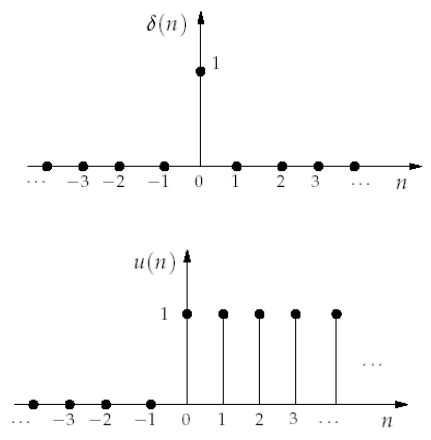
\includegraphics[width=0.38\textwidth]{Lezioni/Immagini/gradinodiscreto}
	\end{center}
	\vspace{-80pt}
\end{wrapfigure}

Esistono anche l'analogo discreto della delta di Dirac e del gradino unitario:
$$\delta(n) = \begin{cases}
1 & \text{se } n = 0 \\
0 & \text{se } n \neq 0
\end{cases}
\qquad
u(n) = \begin{cases}
1 & \text{se } n \geq 0 \\
0 & \text{se } n < 0
\end{cases}$$

$x(n) \cdot \delta(n) = x(0) $ 

$f(n) \cdot \delta(n - n_0) = f(n_0)$ 

$\delta(n) = u(n) - u(n - 1)$

Il gradino continuo, nel discreto diventa una successione di $\delta$: $u(n) = \sum_{i=0}^{+\infty} \delta(n - i)$ 

\section{Sequenze}
Le sequenze $x(n)$ sono formate da segnali a tempo discreto. Se essi sono quantizzati in ampiezza, si parla di segnale digitale. 

\begin{wrapfigure}{R}{0.35\textwidth}
	\vspace{-15pt}
	\begin{center}
		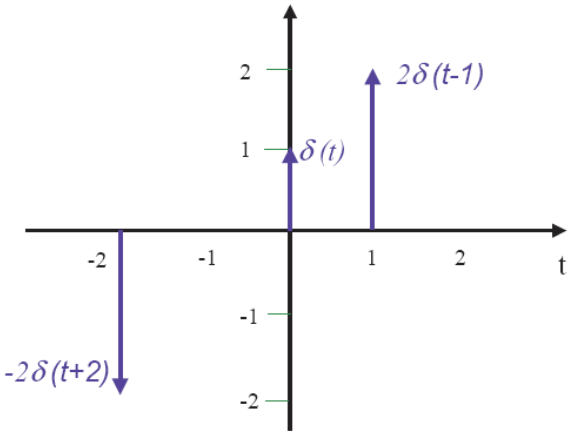
\includegraphics[width=0.3\textwidth]{Lezioni/Immagini/impulso}
	\end{center}
	\vspace{-20pt}
\end{wrapfigure}

Sequenza \textbf{causale}: $x(n) : n > 0$ (con numeri positivi). \\
Sequenza \textbf{anticausale}: $x(n) : n < 0$ (con numeri negativi).

Sequenza \textbf{pari}: $x(n) = x(-n)$ (coseno). \\
Sequenza \textbf{dispari}: $x(n) = -x(-n) \rightarrow x(0) = 0$ (seno).

Sequenza \textbf{periodica}: $x(n) = x(n + T)$ \\
Sequenza \textbf{limitata}: $\abs{x(n)} \leftarrow x_0 < \infty \quad \forall\ n$

Non è possibile tornare indietro nel tempo, quindi le sequenze considerate sono generalmente causali. 

Nella figura, $\delta(n)$ rappresenta l'impulso unitario. Moltiplicando $\delta$ per un coefficiente $k$ l'impulso avrà diversa lunghezza, o diversa direzione se $k$ è negativo. \\
Un ritardo $t - t_0$ sposta l'impulso verso destra, un anticipo $t + t_0$ viceversa.

Se gli impulsi hanno un fattore moltiplicativo $n$, si definisce una funzione \textbf{rampa}: il segnale seguirà la diagonale. 
